\chapter{Future work}
\label{chapter:future}

\subsection{\LSST}

The Large Synoptic Survey Satellite (LSST) is a 8.4 metre telescope with a 9.6
square degree field of view in Cerro Pach\'{o}n, Chile, currently under
construction.
It is designed to observe 18,000 square degrees in the southern sky (south of
+10 degrees, declination) in six Sloan Digital Sky Survey (\SDSS) filters:
{\it ugrizy}.
During its main mode of operation (90\% of the time), \LSST\ will perform two
fifteen second exposures per visit, with one thousand visits per night and
will have a faint limit of around 24.5 in r-band.
For the remaining 10\% of the time, \LSST\ will focus on a small number of
`deep drilling fields'.
These fields are yet to be determined but could be, for example, the Large and
Small Magellanic Clouds, the galactic plane, and so on.
These fields will receive targeted, repeat observations of, for instance 200
observations over a 40-hour period after which the faint limit could be
extended to around 28 apparent magnitudes.
This faint limit will be extended for fields with co-added exposures.
First light is currently scheduled for 2021 and data release one of eleven is
expected to contain eighteen billion objects \citep{Ivezic2008}.

\LSST\ will provide rotation periods for a new stellar regime.
Because \kepler\ targeted Earth-like planet hosts, the majority of its
targets were G stars, with fewer K and M dwarfs.
Since the collecting area of \LSST\ is so large it will be sensitive to a
large number of faint stars, including many K and M dwarfs.
Since it is not a space mission and its lifetime does not depend on the
reliability of moving parts or fuel, \LSST\ will run for 10 years---more than
double the length of the \kepler\ prime mission.
This will open up an opportunity to detect rotation signatures in faint,
slowly rotating stars, allowing us to populate both the low-mass and old parts
of the age-rotation parameter space.
In many ways \LSST\ is \kepler's antithesis: \kepler\ data is dense and evenly
spaced, whereas \LSST\ light curves will have sparse, irregular cadence.
% Depending on its location on the sky, a given target will have between ... and
% ... data points spread over 10 years, spaced from 3 days to 30 days apart.
Most targets will be observed repeatedly for ten years with observations
spaced from three to thirty days apart.
The disadvantage of this is that there will be a rotation period lower limit.
The advantage of using sparse data however, is that CPU time is vastly
reduced!

We simulated \LSST\ cadence by requiring that an object/field only be observed
during the night and whilst the field is visible, so for half of the year.
Each object is visited every three days on average during the observable
season and visits are clustered around a season with a Gaussian shape.
A histogram of the number of visits per week as a function of time for a given
object or field is shown in figure \ref{fig:cadence_hist}.

\begin{figure}
\begin{center}
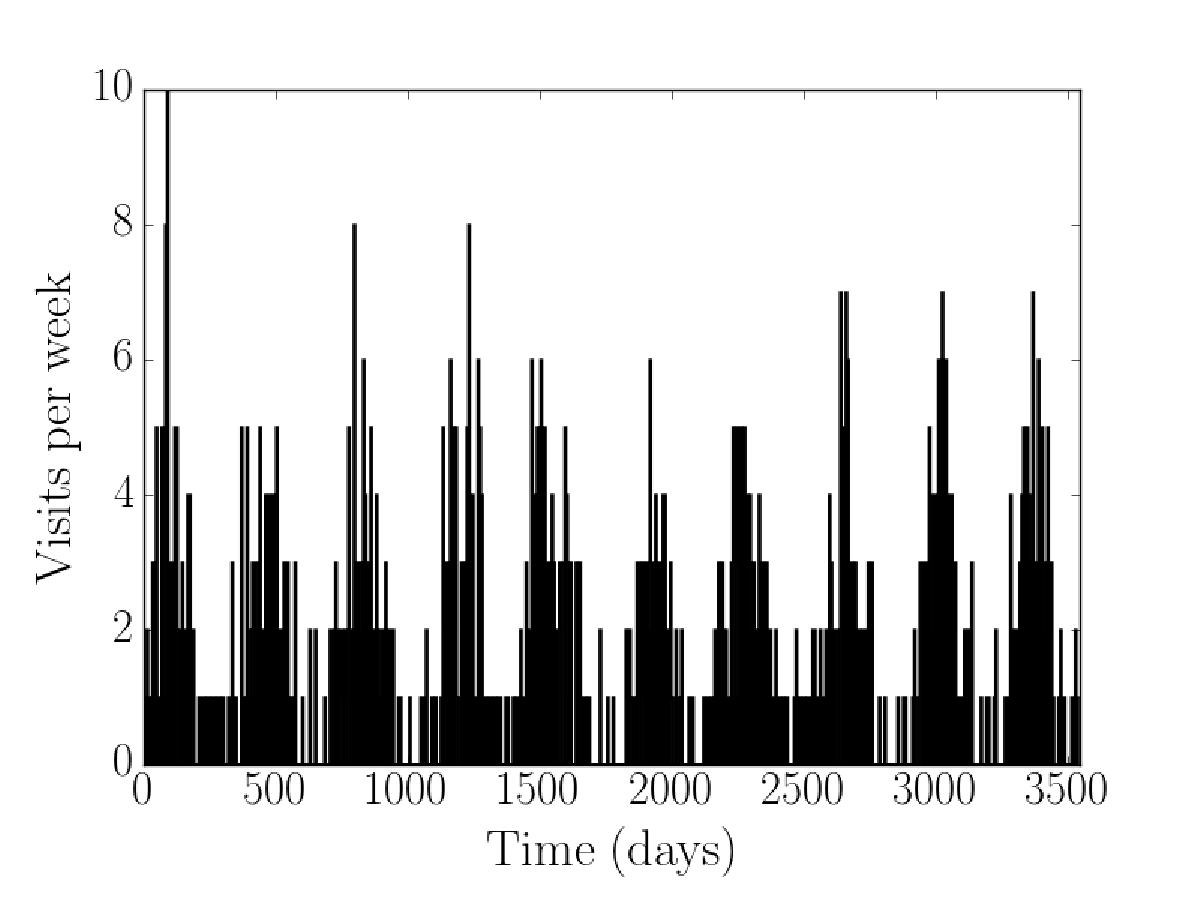
\includegraphics[width=6in, clip=true]{figures/cadence_hist}
\caption[An \LSST\ cadence histogram.]
{A histogram of the number of visits per week as a function of time
for a given object or field observed by \LSST\ as used in our simulations.
Code used to generate this plot was written by Jim Davenport,
\url{https://github.com/jradavenport/MW-Flare}.}
\label{fig:cadence_hist}
\end{center}
\end{figure}

We used the TRILEGAL \citep{Girardi2012} code to simulate stellar populations
in a hypothesised \LSST\ field with galactic coordinates, $l = 45$, $b = -10$.
We randomly selected 5000 stars from this population and with $r$-band
magnitudes between 16 and 28.
We separated these stars into `cool' (< 6250) and `hot' (> 6250) temperature
bins.
For the cool stars we used the new gyrochronology relation, calibrated in
chapter \ref{chapter:gyro} to convert B-V colour (converted from $g-r$) and
age into rotation periods.
% FIXME: include logg
To assign rotation periods to the hot stars we fitted a sum of two Gaussian
functions to the rotation periods of hot stars in the \citet{Mcquillan2014}
catalogue.
We then drew rotation periods from the resulting distribution.
For both hot and cool stars we used code similar to that used in
\citet{Aigrain2015} to simulate light curves, using our theoretical rotation
periods.
In order to assign appropriate amplitudes we approximated the relation between
rotation period, amplitude of variability and \teff, based on the
\citet{Mcquillan2014} sample.
We then assigned amplitudes by drawing values from Gaussians with means
corresponding to the mean amplitudes of stars with similar \teff\ and
$P_{rot}$ in \citet{Mcquillan2014} and variances given by the variance in each
bin.
White noise was added to the light curves, with variance that depended on
$r$-band magnitude, based on the values provided in \citet{Jacklin2015}.
We sampled these light curves using our \LSST\ cadence model and attempted to
recover their rotation periods using a LS periodogram.
Although the LS periodogram has many drawbacks, as explained at length in
previous chapters, an ACF is not useful for \LSST\ data since the data are
unevenly spaced.
We have used the LS periodogram in these initial tests because it is fast to
compute, but intend to use the GP method in the future.

The results are shown in figure \ref{fig:derek}, where recovered rotation
periods are plotted against the rotation periods used to generate the light
curves.
Data points are coloured according to their temperatures.
Rotation periods less than $\sim$ ten days have a low recovery fraction, and
this is worse for hot stars as they have smaller variability amplitudes.
The large outliers at long rotation periods are mostly faint, as shown in
figure \ref{fig:derek2}.

\begin{figure}
\begin{center}
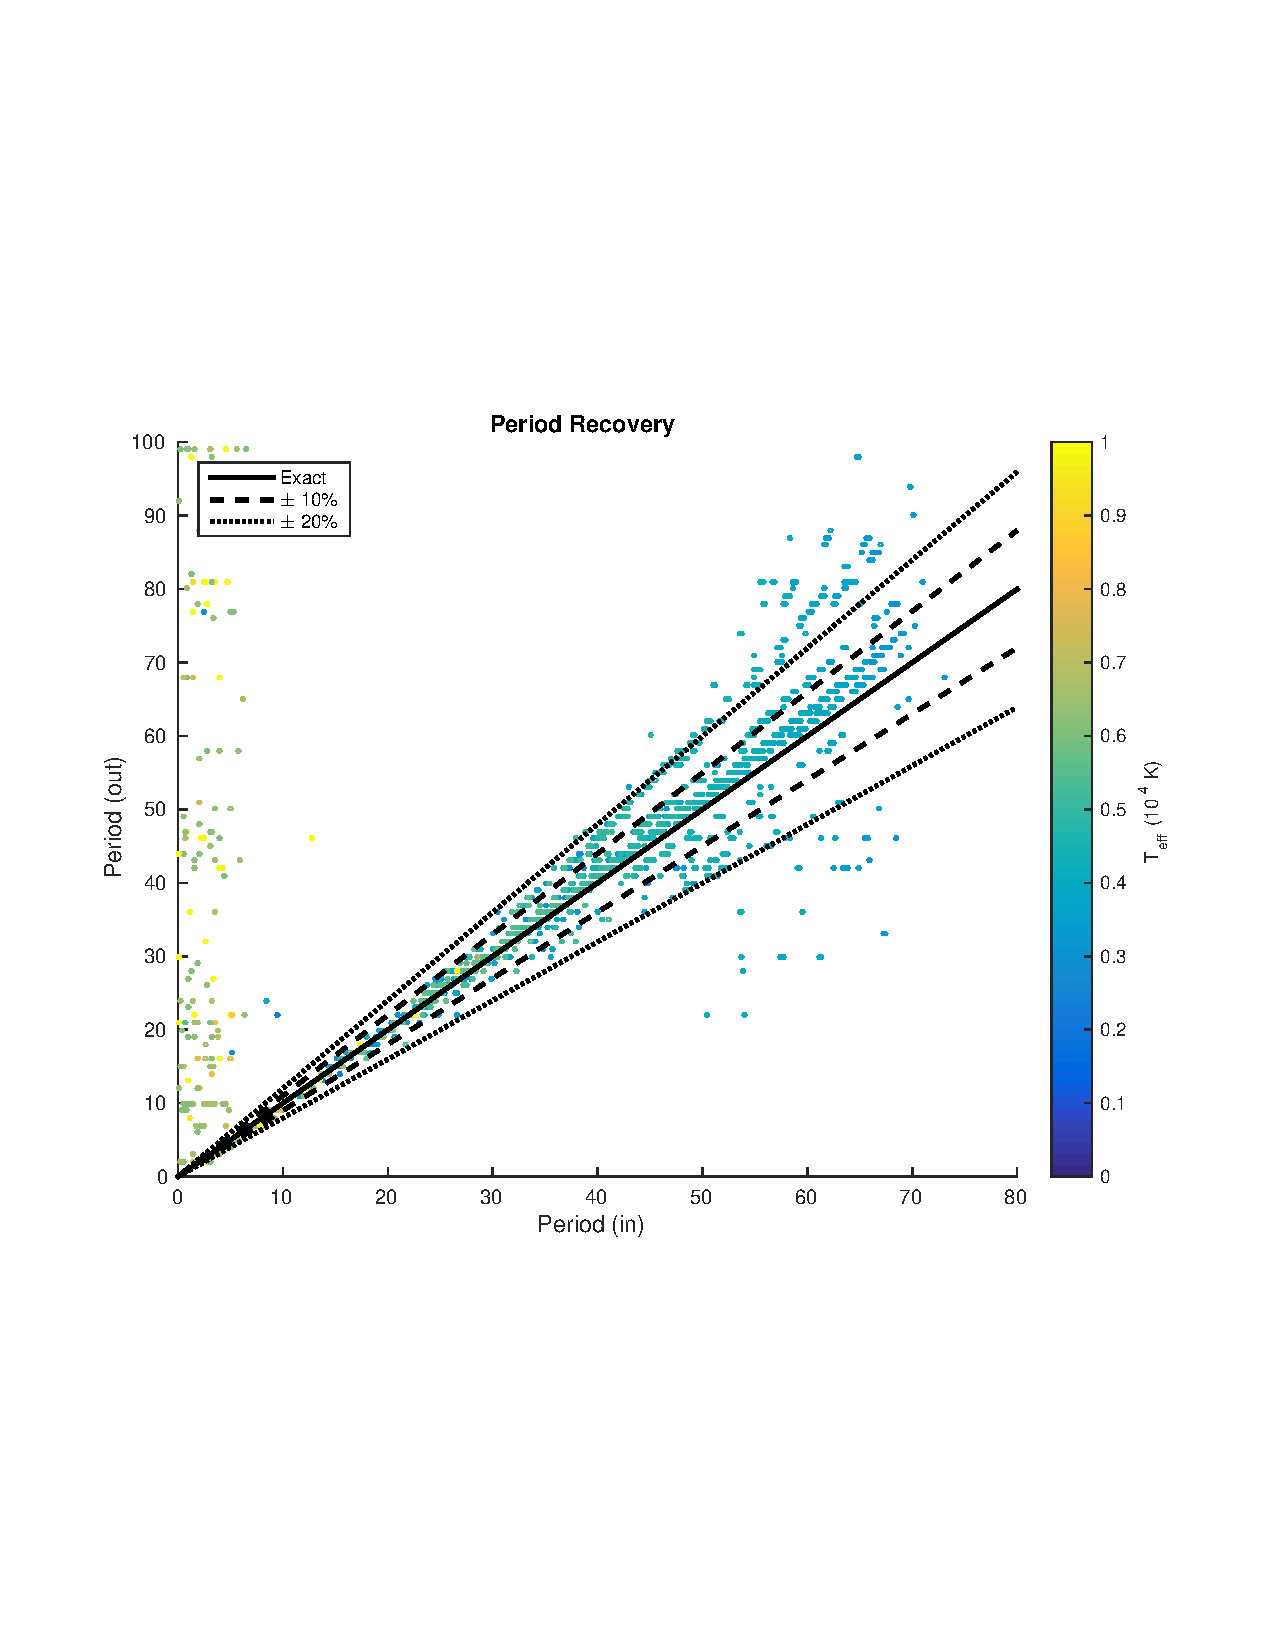
\includegraphics[width=6in, clip=true]{figures/figure6.pdf}
\caption[\LSST\ rotation period recovery results.]
{Measured versus injected rotation period for 5000 simulated \LSST\ targets.
Points are coloured according to their temperatures.
Rotation periods less than $\sim$ 10 days have a low recovery fraction, and
this is worse for hot stars as they have lower amplitudes of variability.
Figure made by Derek Buzazi.}
\label{fig:derek}
\end{center}
\end{figure}

\begin{figure}
\begin{center}
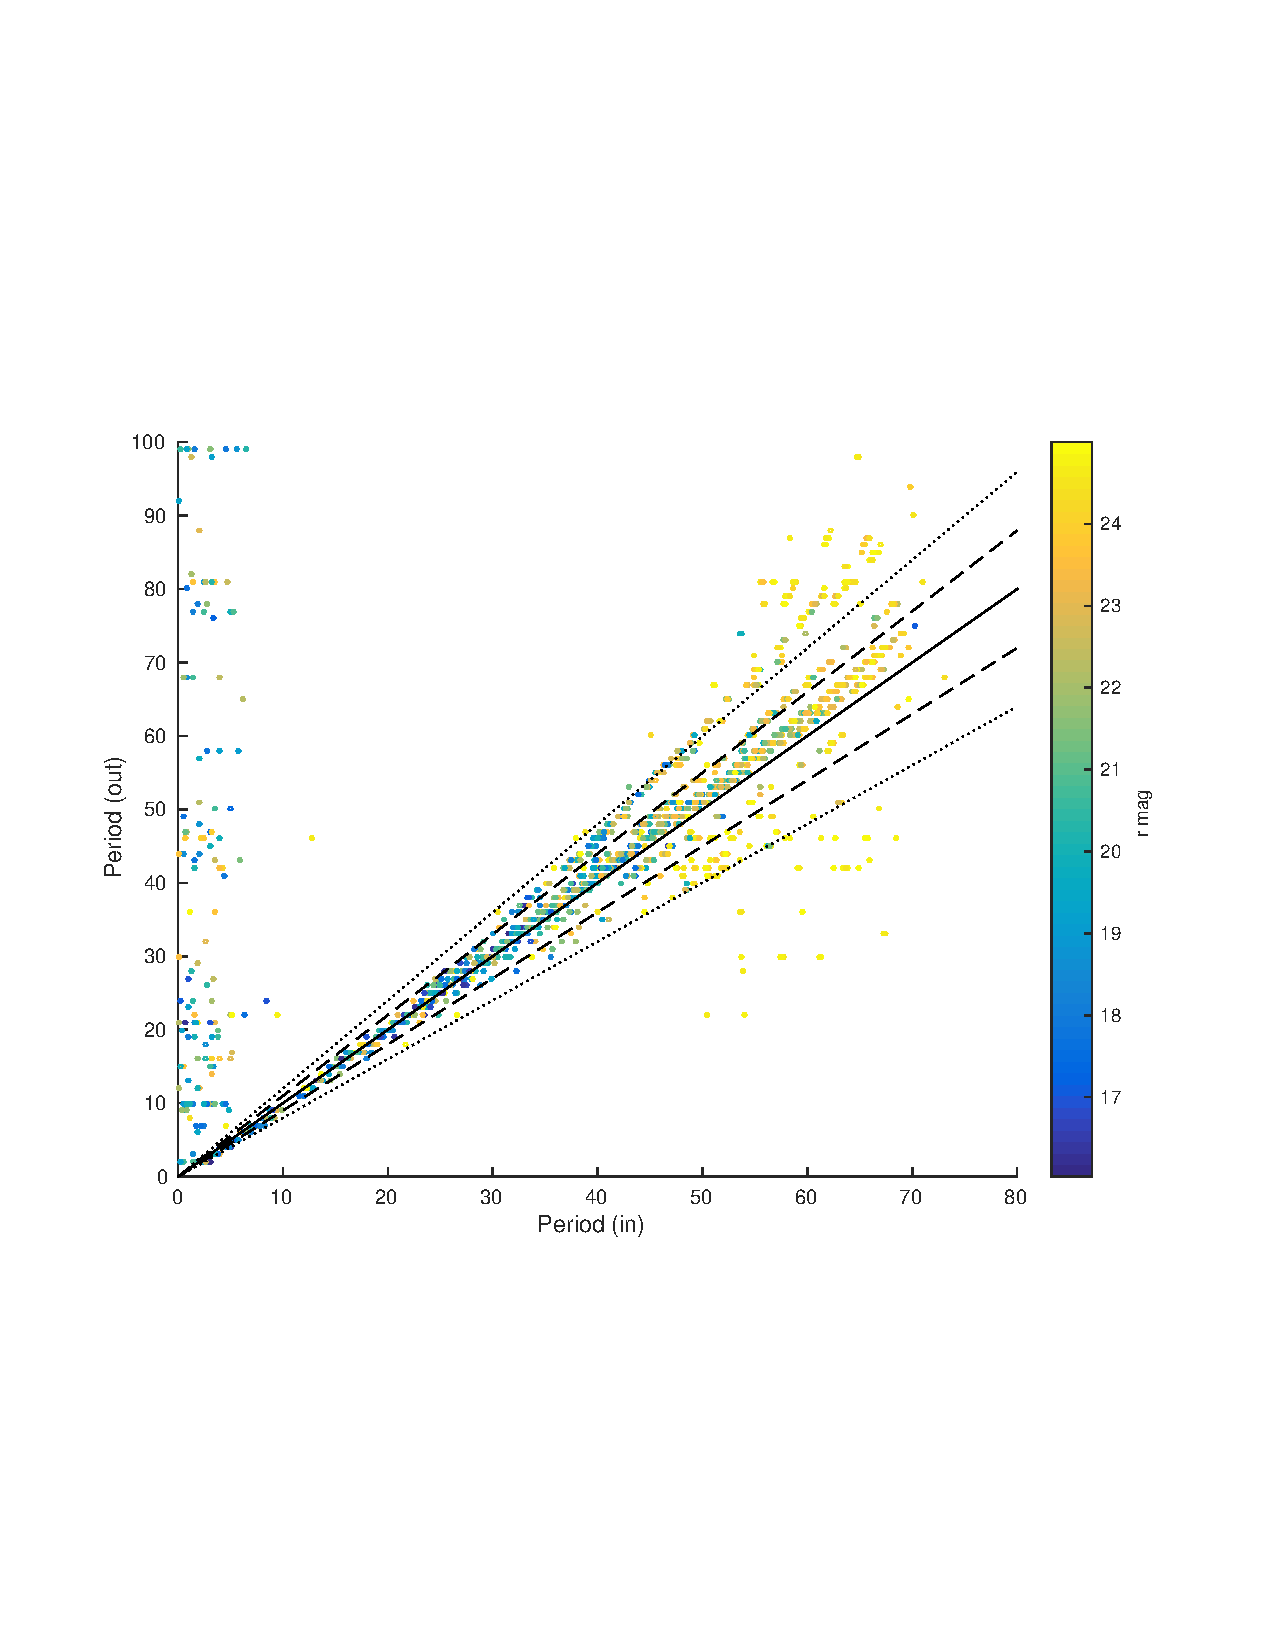
\includegraphics[width=6in, clip=true]{figures/figure8.pdf}
\caption[\LSST\ rotation period recovery results.]
{Measured versus injected rotation period for 5000 simulated \LSST\ targets.
Points are coloured according to the $r$-band magnitude.
The large outliers at long rotation periods are mostly faint.
Figure made by Derek Buzazi.}
\label{fig:derek2}
\end{center}
\end{figure}

This work is the start of an ongoing effort to understand the opportunities
for rotation period recovery in \LSST\ data.
The next steps will be to estimate the total number of rotation periods we
expect to measure from \LSST\ light curves and the types of stars we will be
able to measure them for.
